\begin{figure}[htbp]
\centering
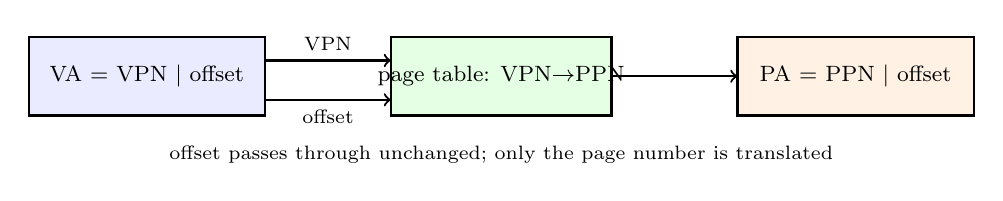
\begin{tikzpicture}[font=\footnotesize, x=1cm, y=1cm]
  \draw[thick, fill=blue!8] (0,2.4) rectangle (3,3.4);
  \node at (1.5,2.9) {VA = VPN $|$ offset};
  \draw[->,thick] (3,3.1) -- (4.6,3.1) node[midway,above]{\scriptsize VPN};
  \draw[->,thick] (3,2.6) -- (4.6,2.6) node[midway,below]{\scriptsize offset};
  \draw[thick, fill=green!10] (4.6,2.4) rectangle (7.4,3.4);
  \node at (6,2.9) {page table: VPN$\to$PPN};
  \draw[->,thick] (7.4,2.9) -- (9.0,2.9);
  \draw[thick, fill=orange!10] (9.0,2.4) rectangle (12,3.4);
  \node at (10.5,2.9) {PA = PPN $|$ offset};
  \node[font=\scriptsize] at (6,1.9) {offset passes through unchanged;
    only the page number is translated};
\end{tikzpicture}
\caption{Translation in one line: the virtual page number becomes a
physical page number through the page table; the offset rides along
untouched. Everything else --- TLBs, walks, faults --- is
engineering around this arrow.}
\label{fig:vapa11}
\end{figure}
